\subsection{Mathematical Tools}\label{subsec:mathematical-tools}

Throughout this paper, we denote vectors and matrices by bold lowercase letters (e.g., $\vecx$) and bold uppercase letters (e.g., $\bm{X}$), respectively.

For $\vecx \in \realNumber^{\intN}$, the mixed $l_{1,2}$ norm is defined as follows:
\begin{equation} \label{eq:L12NormDefinitionEq} \LOneTwoNormDefinition, \end{equation}
where $\mathfrak{G}$ is a set of disjoint index sets, and $\vecx_{\mathfrak{g}}$ is the subvector of $\vecx$ indexed by $\mathfrak{g}$.

For $\vecx \in \realNumber^{\intN}$, the total variation (TV)~\cite{TV} is defined as follows:
\begin{equation} \label{eq:TVDefinitionEq} \TotalVariationDefinition, \end{equation}
where $d_{h,i}$ and $d_{v,i}$ are the horizontal and vertical differences of the $i$-th element of $\vecx$, respectively, when the vector $\vecx$ is considered as a matrix.

\subsection{Proximal Tools}\label{subsec:proximal-tools}
For $\gamma > 0$, $f \in \realNumber^N \to \realNumber$ and $\vecx \in \realNumber^N$, the proximity operator is defined as follows:
\begin{equation} \label{eq:ProximityOperatorDefinitionEq} \proximityOperatorDefinition. \end{equation}

For a proper lower-semicontinuous convex function $f \in \realNumber^N \to \realNumber$ and $\vecx \in \realNumber^N$, the convex conjugate function is defined as follows:
\begin{equation} \label{eq:ConjugateFunctionDefinitionEq} \conjugateFunctionDefinition. \end{equation}

The proximity operator for the convex conjugate function is expressed as follows~\cite[Theorem 3.1 (ii)]{prox-convex-conjugate-function}:
\begin{equation} \label{eq:ProximityOperatorDefinitionWithConvexConjugateFunctionEq} \proximityOperatorDefinitionWithConvexConjugateFunction. \end{equation}

For a set $C \subset \realNumber^N$ and $\vecx \in \realNumber^N$, the indicator function is defined as follows:
\begin{equation} \label{eq:IndicatorFunctionDefinitionEq} \indicatorFunctionDefinition \end{equation}

Define the proximity operator for the indicator function as $P_C$ as follows.
\begin{equation} \label{eq:ProximityOperatorDefinitionWithIndicatorFunctionEq}
\proximityOperator{ \gamma \iota_{C} }{\vecx} = P_C(\vecx) \coloneq \argmin{\vecy \in C} \LTwoNorm{\vecy - \vecx}.
\end{equation}


\subsection{Primal-Dual Splitting Algorithm}\label{subsec:primal-dual-splitting-algorithm}
The Primal-Dual Splitting (PDS) algorithm~\cite{PDS0,PDS1,PDS2,PDS3} is applied to the following problem:
\begin{equation} \label{eq:PDSPrimalEq} \PDSPrimal, \end{equation}
where $\bm{L} \in \realNumber^{\intM \times \intN}$, $f$ is a differentiable convex function and $g,h$ are convex functions whose proximity operator can be computed efficiently.

The PDS algorithm solves prob.~\eqref{eq:PDSPrimalEq} by iteratively updating the following:
\begin{equation} \label{eq:PDSSubStep} \PDSSubStep \end{equation}
where $\gamma_1, \gamma_2 \in \realNumber$ are step sizes.


\begin{figure*}[htbp]
    \centering
    \begin{tabular}{m{118mm} m{10mm} m{0mm}}
        \begin{minipage}[b]{120mm}
            \centering
            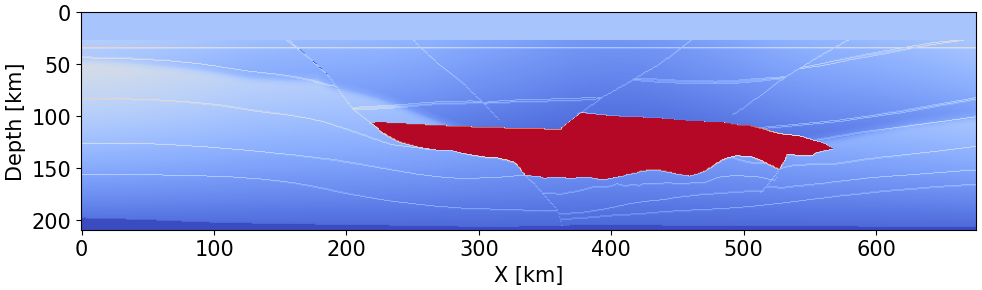
\includegraphics[width=120mm]{public/full_true_vm}
        \end{minipage} &
        \begin{minipage}[b]{20mm}
            \centering
            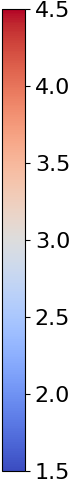
\includegraphics[height=36mm]{public/color-bar}
        \end{minipage} &
    \end{tabular}
    \caption{the velocity model of the Salt [km/s]}
    \label{fig:salt-model}
\end{figure*}



\subsection{Full Waveform Inversion}\label{subsec:full-waveform-inversion}
Typically, FWI is treated as an optimization problem as follows\cite{FWI0}:
\begin{equation} \label{eq:FWIObjective} \argmin{\velModel \in \realNumber^N} \ \ \FWIObjectiveDefinition, \end{equation}
where $\velModel \in \realNumber^{N}$ is the velocity model representing subsurface properties, $\seismicData_{\mathrm{obs}} \in \realNumber^{M}$ is the observed seismic data, $\seismicData_{\mathrm{cal}}$ is the observation process, and $\seismicData_{\mathrm{cal}(\velModel)}$ is the modeled seismic data with the velocity model.
$N$ is the number of grid points, and $M$ is the number of observed signals.
In general, the velocity model is 2D or 3D grid data, but for simplicity we consider flattened 1D vector.

The observation process $\seismicData_{\mathrm{cal}}$ is nonlinear and complex, making it difficult to express analytically.
However, the gradient $\nabla E$ can be computed numerically using the adjoint-state method~\cite{FWI-gradient}.

Therefore, the standard FWI minimizes the objective function and reconstructs the velocity model using the following procedures:
\begin{equation} \label{eq:FWIWithGradient} \FWIWithGradient, \end{equation}
where $\gamma$ is the step size.

